\documentclass{article}
\usepackage{amsmath}
\usepackage{amssymb}
\usepackage{graphicx}
\usepackage{hyperref}
\usepackage[version=4]{mhchem}


\begin{document}
Given a triangle \(A B C\) and its medians \(A D, B E\), and \(C F\), construct a triangle with sides of length \(A D, B E\), and \(C F\). Show that the area of the triangle of medians is three-fourths of the area of the given triangle.\\
\centering
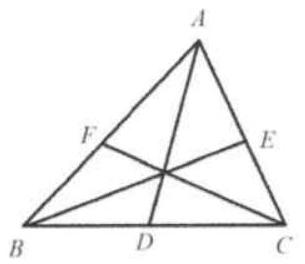
\includegraphics[width=\textwidth]{images/040(2).jpg}


Solution:
Extend \(F E\) to \(H\) such that \(E H=D C=\frac{1}{2} B C\). Connect \(H D, H A, H C\).\\
Since \(E F\) is the midline of triangle \(A B C, E F / / B C\), and \(E F=\frac{1}{2} B C\).\\
Thus \(F H / / B C\), and \(F H=B C\), then \(H C B F\) is a parallelogram. So \(H C / / B F\), and \(H C=B F\). So \(H C / / A F\), and \(H C=A F\). Thus \(C H A F\) is a parallelogram. So \(A H=\) \(C F\).\\
Since \(E H / / B D\), and \(E H=B D, H D B E\) is a parallelogram.\\
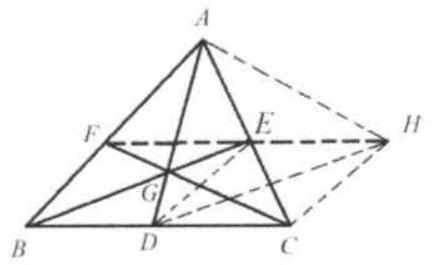
\includegraphics[width=\textwidth]{images/041.jpg} So \(H D=B E\).

This tells us that triangle \(A D H\) is a triangle with three sides of \(A D, B E . C F\). Now connect \(D E\).\\
Since \(E D\) is the midline of triangle \(A B C, E D / / A B\), and \(E D=\frac{1}{2} A B\) and \(S_{\triangle E D A}=\frac{1}{2} S_{\triangle A D C}=\frac{1}{4} S_{\triangle A B C}\).\\
We know that \(H D B E\) is a parallelogram, so \(S_{\triangle E D H}=S_{\triangle E B D}=\frac{1}{2} S_{\triangle E B C}=\frac{1}{4} S_{\triangle A B C}\)\\
We also know that \(H C F A\) is a parallelogram, so\\
\(S_{\triangle E A H}=S_{\triangle E F C}=\frac{1}{2} S_{\triangle A F C}=\frac{1}{4} S_{\triangle A B C}\).\\
Therefore, \(S_{\triangle A D H}=S_{\triangle E D H}+S_{\triangle E H A}+S_{\triangle E A D}=\frac{3}{4} S_{\triangle A B C}\).\\

\end{document}
